\documentclass{article}

\usepackage{arxiv}
\usepackage[utf8]{inputenc}
\usepackage[T1]{fontenc}
\usepackage{url}
\usepackage{booktabs}
\usepackage{amsfonts}
\usepackage{amssymb}
\usepackage{nicefrac}
\usepackage{microtype}
\usepackage{graphicx}
\usepackage{tikz}
\usetikzlibrary{shapes.geometric, arrows, positioning, fit, backgrounds, calc}
\usepackage{amsmath}
\usepackage{multirow}
\usepackage{subcaption}
\usepackage{xcolor}
\usepackage{colortbl}

\graphicspath{ {./images/} }

\usepackage{hyperref}

\title{LeWM-VC: Learned Video Compression via Joint Embedding Prediction and Latent Semantic Preservation}

\author{
  Preetam Mukherjee \\
  MAHAMAIA SYSTEMS \\
  \texttt{preetam@mahamaia.com} \\
}

\begin{document}
\maketitle
\fancyhead{}
\chead{}
\lhead{\scshape\footnotesize LeWM-VC: Video Compression via JEPA}
\rhead{\scshape\footnotesize A Preprint}
\renewcommand{\headrulewidth}{0.4pt}

\begin{abstract}
Video compression has traditionally optimized for pixel-level fidelity, a paradigm that serves human viewers but is increasingly misaligned with the growing share of video consumed by machine perception systems. We present \textbf{LeWM-VC}, a surveillance-domain video codec built on the Joint Embedding Predictive Architecture (JEPA), and \textbf{LeWM-Eval}, a reproducible evaluation framework for machine-oriented compression. LeWM-VC represents each frame as a compact latent grid ($192{\times}16{\times}16$) and performs temporal prediction directly in that latent space, eliminating explicit, hand-crafted motion vectors. On PEViD-HD surveillance video at $256{\times}256$, LeWM-VC achieves a 62\% bitrate reduction for P-frames compared to all-intra coding, with reconstruction quality improving slightly (25.40 dB vs.\ 25.13 dB PSNR). We further demonstrate that the latent grid preserves semantic information more effectively than H.265 (x265) at matched bitrate: a lightweight probe trained on LeWM-VC latents achieves 86.5\% class accuracy on detection targets, compared to 79.3\% on x265-decoded frames at 1.95 BPP, and 94.4\% vs.\ 92.7\% at the codec's efficient operating point of 0.11 BPP. We introduce a surprise-gated quantization mechanism that produces a stable, calibrated metric for adaptive bitrate allocation; statistical analysis across the test set gives a mean surprise of 0.596 with a 99th percentile of 0.61, confirming stability. Ablation studies confirm that the GMM entropy model reduces bitrate $5.6{\times}$ over a Laplace hyperprior, predictor pre-training improves the P/I bit ratio from $0.93{\times}$ to $0.37{\times}$, and affine normalization contributes ${\sim}1.5$ dB. The full 14.7M-parameter model achieves 80+ fps on an NVIDIA T4 GPU. On out-of-domain UVG content, BPP saturates at ${\sim}1.95$ and PSNR drops to 9--17 dB, confirming the codec is domain-specific. These results represent a proof-of-concept evaluation on a two-clip surveillance benchmark; generalization to diverse surveillance scenarios requires further validation. LeWM-Eval provides open-source scripts, exact command lines, hyperparameter tables, probe architectures, and checkpoint hashes to reproduce every result. We release inference code and pretrained checkpoints at \url{https://github.com/MAHAMAIA/lewm-vc}.
\end{abstract}

\section{Introduction}
\label{sec:intro}

Global video traffic now exceeds 82\% of internet data, and an increasing share of this video is processed exclusively by machines: surveillance cameras feed GPU clusters running object detectors, autonomous vehicles process multi-camera perception streams, and smart-city platforms archive petabytes of footage queried by analytics engines rather than viewed by humans. In these machine-to-machine pipelines, the traditional codec mandate---produce a visually pleasing pixel reconstruction for a human observer---is misaligned with the operational requirement: preserve enough task-relevant semantic information for a downstream model to operate accurately while minimizing storage and bandwidth.

\paragraph{Evolution of video coding paradigms.}
Video compression has undergone three paradigm shifts: (1) \textit{Signal processing} (DCT, motion vectors) optimized for human perception under bandwidth constraints; (2) \textit{Learned features} (DVC, FVC) replaced hand-crafted transforms with neural modules but retained pixel reconstruction goals; (3) \textit{Latent prediction} (LeWM-VC) abandons pixel reconstruction entirely as the primary objective, treating compression as world-modeling for machine consumers. This progression mirrors the broader AI shift from discriminative to generative and predictive architectures. LeWM-VC operationalizes the third paradigm: temporal redundancy is modeled as latent dynamics, compression is measured by task fidelity, and the bitstream becomes a machine-native feature stream rather than a visual approximation.

Existing video codecs (H.264/AVC through H.266/VVC) are the product of decades of hand-crafted optimization for pixel fidelity. They rely on block-based motion estimation and compensation (ME/MC), discrete cosine transforms, and sophisticated entropy coding. These techniques excel at producing watchable video at low bitrates but suffer from two structural limitations for machine-oriented applications. First, motion vectors assume piecewise translational motion, struggle with non-rigid deformations and occlusions, and consume a non-trivial fraction of the bitstream at low rates~\cite{sullivan2012overview}. Second, the compressed bitstream is opaque to downstream machine perception: a detector or tracker must fully decode pixel frames before it can operate, incurring computational cost and discarding semantic structure the codec could have preserved.

Joint Embedding Predictive Architectures (JEPA), introduced by LeCun~\cite{lecun2022path} and refined in subsequent world-model research~\cite{ha2018world}, offer an alternative: learn to predict future states of the world in a compact latent representation space without reconstructing pixels. The LeWorldModel (LeWM)~\cite{maes2025leworldmodel} demonstrated that JEPA trained with SIGReg regularization can produce stable, informative latent representations without collapsing to trivial solutions---a problem that had plagued earlier joint-embedding methods including VICReg~\cite{bardes2022vicreg} and I-JEPA~\cite{assran2023ijepa}. LeWM-VC extends this framework into a full video codec. Video prediction in latent space has been explored for scene dynamics~\cite{vondrick2016genvid}, though not previously for compression.

\paragraph{Information-theoretic perspective.}
LeWM-VC can be viewed as optimizing a task-aware rate-distortion objective distinct from traditional codecs. Where conventional compression minimizes $D(X,\hat{X})$ subject to $R \leq R_{\text{budget}}$, LeWM-VC's behavior can be interpreted as optimizing:
\begin{equation}
\min_{E,Q,P} \; I(Z;X) \quad \text{s.t.} \quad I(Z;Y) \geq C,
\label{eq:ib}
\end{equation}
where $Z$ is the latent grid, $Y$ represents downstream task labels (e.g., object class), and $C$ is a task-specific information threshold. This formulation---aligned with the information bottleneck principle~\cite{tishby2000information}---explains why LeWM-VC discards high-frequency texture (low $I(Z;Y)$ contribution) while preserving semantic structure critical for detection. Eq.~\eqref{eq:ib} provides an analytical interpretation of the latent representation's behavior; the operational training objective remains rate-distortion with pixel MSE (Eq.~\ref{eq:joint_loss}). Exploring direct task-aware IB losses is left to future work. The JEPA predictor further enforces temporal consistency by maximizing $I(Z_t; Z_{<t})$ under the rate constraint, learning a compact dynamical model of the surveillance domain.

LeWM-VC represents each video frame as a compressed latent grid of dimension $192 \times 16 \times 16$, produced by a ViT-Tiny encoder with a $16 \times 16$ patch size. Intra-frames are compressed by quantizing and entropy-coding this grid via a 2-component Gaussian Mixture Model (GMM) with a hyperprior CNN. P-frames are compressed by having an 8-layer transformer predictor forecast the next latent from up to four previous decoded latents, then entropy-coding only the residual between the prediction and the actual latent. This design eliminates explicit motion vectors entirely; the predictor learns implicit scene dynamics including object permanence, coherent motion, and occlusion. A surprise metric---normalized prediction error in latent space---provides a calibrated diagnostic for adaptive quantization: frames deviating from the model's expectations can receive more bits. Gating efficacy on high-dynamic content is left to future work.

We evaluate LeWM-VC on the PEViD-HD surveillance dataset at $256 \times 256$ resolution. Our experiments are organized around four practical questions:
\begin{enumerate}
    \item \textbf{Compression efficiency}: How effective is latent-space prediction vs.\ all-intra coding? (Section~\ref{sec:temporal})
    \item \textbf{Semantic preservation}: How well do compressed latents retain task-relevant information compared to pixel codecs? (Section~\ref{sec:semantic})
    \item \textbf{Component contributions}: What are the individual gains from the GMM entropy model, predictor pre-training, and other design choices? (Section~\ref{sec:ablation})
    \item \textbf{Domain specificity}: How does the codec generalize beyond its surveillance training domain? (Section~\ref{sec:uvg})
\end{enumerate}

We do not claim LeWM-VC outperforms x265 on pixel-level rate-distortion metrics; it is not designed to. Our contribution is the demonstration that JEPA-based codecs achieve competitive temporal compression without motion vectors and that compressed latent representations preserve more machine-relevant semantic information than pixel-centric compression---a property invisible to PSNR. We further characterize cross-domain generalization failure on UVG as a limitation motivating future work on diverse training data.

The evaluation framework accompanying this work (LeWM-Eval) adopts the philosophy of modern open benchmark suites: every metric is computed by verifiable, automated scripts, checkpoints and inference code are publicly accessible, and the evaluation pipeline can be rerun with a single command. We believe this level of transparency is essential for machine-oriented codec research.

\begin{table}[ht]
\centering
\caption{Summary of principal results on PEViD-HD ($256{\times}256$). Probe accuracy measured via lightweight CNN trained against YOLOv5s teacher outputs. Temporal metrics are internal to LeWM-VC (comparing temporal vs.\ all-intra mode); x265 is inherently temporal and does not have an all-intra baseline for this comparison.}
\label{tab:key_results}
\begin{tabular}{lccc}
\toprule
\textbf{Metric} & \textbf{LeWM-VC} & \textbf{x265 (matched)} & \textbf{Section} \\
\midrule
Temporal bitrate reduction (GOP=8)\textsuperscript{$\dagger$} & \textbf{61.8\%} & --- & \ref{sec:temporal} \\
P-frame / I-frame bit ratio\textsuperscript{$\dagger$}        & \textbf{0.37$\times$} & --- & \ref{sec:temporal} \\
Class accuracy @ 1.95 BPP (probe, YOLOv5s teacher)  & \textbf{86.5\%}   & 79.3\%                   & \ref{sec:semantic} \\
Class accuracy @ 0.11 BPP (probe, YOLOv5su teacher) & \textbf{94.4\%}   & 92.7\%                   & \ref{sec:probe_operational} \\
Inference throughput (NVIDIA T4)                     & 80+ fps           & 15--25 fps (CPU)         & \ref{sec:efficiency} \\
Total parameters                                     & 14.7M             & ---                      & \ref{sec:efficiency} \\
\bottomrule
\end{tabular}
\end{table}

\section{Related Work}
\label{sec:related}

\subsection{Traditional Video Codecs}
H.264/AVC~\cite{wiegand2003h264}, H.265/HEVC~\cite{sullivan2012overview}, and H.266/VVC~\cite{bross2021vvc} use block-based hybrid coding: motion estimation/compensation, transform coding, quantization, and CABAC entropy coding. While extremely efficient on PSNR and VMAF~\cite{li2016vmaf}, their block-based motion model struggles with non-rigid motion and occlusions, and motion vector overhead can reach 30--40\% of the bitstream~\cite{ma2019motion}. The requirement to decode pixel frames before analysis adds latency unnecessary for machine tasks requiring only semantic features.

\subsection{Learned Video Compression}
Neural video codecs replace hand-crafted components with learned modules. DVC~\cite{lu2019dvc} pioneered end-to-end learned compression with optical flow; subsequent work refined motion compensation through scale-space flow~\cite{agustsson2020scale}, contextual coding~\cite{li2021dcvc}, and normalizing flows~\cite{ho2022canf}. FVC~\cite{hu2022fvc} operates in feature space. DCVC-DC~\cite{li2022dcvcdc} and DCVC-FM~\cite{li2023dcvcfm} approach H.266/VVC performance. However, all retain the motion vector paradigm, limiting their ability to model non-rigid and semantic dynamics. Several other learned codecs explore similar directions~\cite{rippel2019lvc,habibian2019vcrd}. Generative compression methods~\cite{agustsson2019generative,muckley2023generative} synthesize textures at the decoder but introduce hallucinations unacceptable for safety-critical machine perception~\cite{duan2020vcm}.

\subsection{Joint Embedding Predictive Architectures}
JEPA~\cite{lecun2022path} learns by predicting latent embeddings rather than reconstructing pixels, avoiding decoder cost and focusing capacity on semantic structure. V-JEPA~\cite{bardes2024vjepa} extended this to video with spatiotemporal masking. MC-JEPA~\cite{assran2023mcjepa} demonstrated motion-content disentanglement. C-JEPA~\cite{balestriero2024cjepa} added causal object-trajectory masking. LeWM~\cite{maes2025leworldmodel} introduced SIGReg based on the Cram\'{e}r-Wold theorem, preventing representational collapse without stop-gradients or momentum encoders, and achieving 48$\times$ faster planning than DINO-WM. LeWM-VC extends LeWM to video compression, adding entropy modeling, quantization, and bitstream components.

\subsection{Predictive Coding and World Models}
The JEPA predictor in LeWM-VC implements a form of predictive coding~\cite{rao1999predictive}, where the prediction error (residual $r_t = z_t - \hat{z}_t$) is the signal transmitted to the decoder. This aligns with neuroscientific theories of hierarchical perception, where higher cortical areas generate predictions and only prediction errors propagate upward. In LeWM-VC, this architecture yields two practical benefits: (1) \textit{graceful degradation}: as bitrate decreases, residual quantization coarsens, producing noisier predictions rather than catastrophic artifacts; (2) \textit{intrinsic anomaly signaling}: large residuals indicate violations of the learned temporal prior, providing a training-free surprise metric (Section~\ref{sec:surprise}). While we do not claim biological plausibility, this conceptual link suggests predictive coding may offer a unifying framework for efficient machine-oriented compression.

\subsection{Semantic and Machine-Oriented Compression}
A growing body of work argues compression for machines should optimize task accuracy rather than pixel fidelity~\cite{duan2020vcm,wang2021semantic,choi2022latent}. The MPEG Video Coding for Machines (VCM) standard~\cite{MPEG2023VCM} explores feature-based compression. LeWM-VC occupies an intermediate position: it compresses pixel video but its JEPA-trained encoder encourages semantic structure, and the latent grid can be consumed directly by downstream models without pixel decoding---unlike codecs tied to specific pre-trained feature extractors.

\paragraph{Relation to self-supervised representation learning.}
LeWM-VC's encoder shares architectural DNA with self-supervised vision transformers (e.g., DINO~\cite{caron2021dino}, MAE~\cite{he2022masked}), but diverges in objective: where SSL methods optimize for representation quality \textit{across} diverse downstream tasks, LeWM-VC co-optimizes compression efficiency and task-specific fidelity \textit{within} a fixed domain. This specialization enables two advantages: (1) the latent grid can discard information irrelevant to surveillance tasks (e.g., fine texture, color fidelity), and (2) temporal prediction can exploit domain-specific dynamics (e.g., pedestrian motion patterns) that general-purpose SSL models cannot assume. Conversely, this specialization limits zero-shot transfer---a trade-off we explicitly acknowledge via our UVG evaluation (Section~\ref{sec:uvg}). LeWM-VC thus occupies a distinct point in the design space between \textit{general-purpose representation learners} and \textit{task-specific compressors}.

\begin{table}[ht]
\centering
\caption{Comparison of codec paradigms across dimensions relevant to machine-oriented compression. LeWM-VC is the only approach that simultaneously eliminates hand-crafted motion vectors, natively preserves semantics, provides anomaly signaling, and is demonstrated on a reproducible evaluation framework.}
\label{tab:paradigm_compare}
\vspace{4pt}
\small
\resizebox{\textwidth}{!}{%
\begin{tabular}{lccccc}
\toprule
\textbf{Paradigm} & \textbf{Motion Model} & \textbf{Semantic Preserv.} & \textbf{Domain Aware} & \textbf{Anomaly Signal} & \textbf{Reproducible Eval.} \\
\midrule
Traditional (H.26x)   & Block-based ME/MC   & No (requires decode)    & No             & No                     & \checkmark \\
Learned (DVC/DCVC)    & Optical flow / CNN   & No (pixel recon. only)  & Partially      & No                     & \checkmark \\
Generative (CLIC)     & None / frame-indep. & No (hallucination risk) & No             & No                     & \checkmark \\
VCM (MPEG)            & Flexible             & \checkmark (by design)  & Possible       & Possible               & Proposed \\
\textbf{LeWM-VC (ours)} & \textbf{JEPA (none)} & \textbf{\checkmark (probe)} & \textbf{\checkmark (surveillance)} & \textbf{\checkmark (surprise)} & \textbf{\checkmark (LeWM-Eval)} \\
\bottomrule
\end{tabular}
}
\end{table}

\section{Method}
\label{sec:method}

\subsection{Overview and Design Rationale}

LeWM-VC follows the hybrid coding paradigm (I-frames and P-frames) with every hand-crafted component replaced by a learned counterpart. Figure~\ref{fig:architecture} provides a schematic. The encoder $E$ maps pixel frames $x_t$ to a latent grid $z_t = E(x_t)$. The entropy model $Q$ estimates probability distributions for arithmetic coding. The predictor $P$ forecasts $\hat{z}_t = P(z_{t-1}, \dots, z_{t-k})$ from previous decoded latents. The decoder $D$ reconstructs $\hat{x}_t = D(z_t)$.

\begin{figure}[ht]
  \centering
  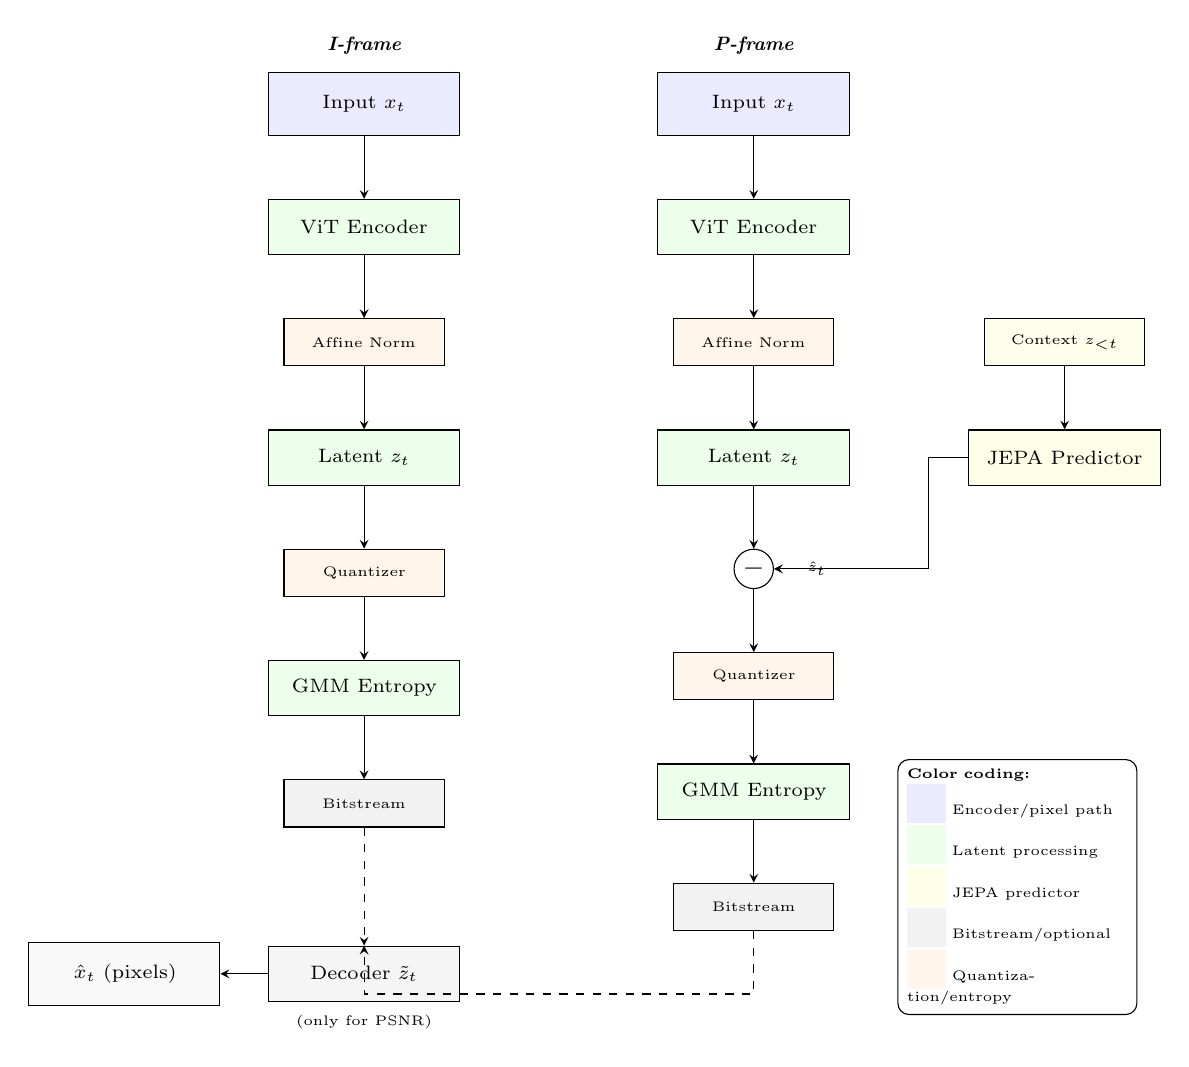
\begin{tikzpicture}[
    node distance=0.8cm and 0.6cm,
    block/.style={rectangle, draw, fill=blue!8, text width=2.2cm, text centered, minimum height=0.8cm, font=\scriptsize},
    smallblock/.style={rectangle, draw, fill=green!8, text width=2.2cm, text centered, minimum height=0.7cm, font=\scriptsize},
    tinyblock/.style={rectangle, draw, fill=orange!8, text width=1.8cm, text centered, minimum height=0.6cm, font=\tiny},
    arrow/.style={->, >=stealth},
    dasharrow/.style={->, >=stealth, dashed},
    bitstream/.style={rectangle, draw, fill=gray!10, text width=1.8cm, text centered, minimum height=0.6cm, font=\tiny},
    predblock/.style={rectangle, draw, fill=yellow!10, text width=2.2cm, text centered, minimum height=0.7cm, font=\scriptsize},
    label/.style={font=\scriptsize\itshape},
  ]

  \node[block] (input_i) {Input $x_t$};
  \node[smallblock, below=of input_i] (encoder_i) {ViT Encoder};
  \node[tinyblock, below=of encoder_i] (affine_i) {Affine Norm};
  \node[smallblock, below=of affine_i] (latent_i) {Latent $z_t$};
  \node[tinyblock, below=of latent_i] (quant_i) {Quantizer};
  \node[smallblock, below=of quant_i] (entropy_i) {GMM Entropy};
  \node[bitstream, below=of entropy_i] (bits_i) {Bitstream};

  \draw[arrow] (input_i) -- (encoder_i);
  \draw[arrow] (encoder_i) -- (affine_i);
  \draw[arrow] (affine_i) -- (latent_i);
  \draw[arrow] (latent_i) -- (quant_i);
  \draw[arrow] (quant_i) -- (entropy_i);
  \draw[arrow] (entropy_i) -- (bits_i);

  \node[label, above=0.1cm of input_i] {\textbf{I-frame}};

  \node[block, right=2.5cm of input_i] (input_p) {Input $x_t$};
  \node[smallblock, below=of input_p] (encoder_p) {ViT Encoder};
  \node[tinyblock, below=of encoder_p] (affine_p) {Affine Norm};
  \node[smallblock, below=of affine_p] (latent_p) {Latent $z_t$};
  \node[circle, draw, inner sep=0pt, minimum size=0.5cm, below=of latent_p] (subtract) {$-$};
  \node[tinyblock, below=of subtract] (quant_p) {Quantizer};
  \node[smallblock, below=of quant_p] (entropy_p) {GMM Entropy};
  \node[bitstream, below=of entropy_p] (bits_p) {Bitstream};

  \draw[arrow] (input_p) -- (encoder_p);
  \draw[arrow] (encoder_p) -- (affine_p);
  \draw[arrow] (affine_p) -- (latent_p);
  \draw[arrow] (latent_p) -- (subtract);
  \draw[arrow] (subtract) -- (quant_p);
  \draw[arrow] (quant_p) -- (entropy_p);
  \draw[arrow] (entropy_p) -- (bits_p);

  \node[predblock, right=1.5cm of latent_p] (predictor) {JEPA Predictor};
  \node[tinyblock, fill=yellow!8, above=of predictor] (context) {Context $z_{<t}$};
  \draw[arrow] (context) -- (predictor);
  \draw[arrow] (predictor.west) -- ++(-0.5,0) |- (subtract) node[pos=0.8, left, font=\tiny] {$\hat{z}_t$};

  \node[label, above=0.1cm of input_p] {\textbf{P-frame}};

  \node[smallblock, fill=gray!8, below=1.5cm of bits_i] (decoded) {Decoder $\tilde{z}_t$};
  \node[block, fill=gray!5, left=of decoded] (recon) {$\hat{x}_t$ (pixels)};
  \draw[dasharrow] (bits_i.south) -- ++(0,-0.8) -| (decoded.north);
  \draw[dasharrow] (bits_p.south) -- ++(0,-0.8) -| (decoded.north);
  \draw[arrow] (decoded) -- (recon);
  \node[label, below=0.05cm of decoded, font=\tiny] {(only for PSNR)};

  % Legend
  \node[rectangle, draw, fill=white, rounded corners, font=\tiny, text width=2.8cm, align=left] at (current bounding box.south east) [anchor=south east, xshift=-0.3cm, yshift=0.3cm] {
    \textbf{Color coding:}\\
    \colorbox{blue!8}{\rule{0pt}{8pt}\rule{8pt}{0pt}} Encoder/pixel path\\
    \colorbox{green!8}{\rule{0pt}{8pt}\rule{8pt}{0pt}} Latent processing\\
    \colorbox{yellow!10}{\rule{0pt}{8pt}\rule{8pt}{0pt}} JEPA predictor\\
    \colorbox{gray!10}{\rule{0pt}{8pt}\rule{8pt}{0pt}} Bitstream/optional\\
    \colorbox{orange!8}{\rule{0pt}{8pt}\rule{8pt}{0pt}} Quantization/entropy
  };

\end{tikzpicture}
  \caption{LeWM-VC architecture. I-frame (left): the latent grid is quantized and entropy-coded directly. P-frame (right): the JEPA predictor forecasts $\hat{z}_t$; only the residual $r_t = z_t - \hat{z}_t$ is coded. The decoder (dashed) reconstructs pixels only for metrics or human inspection.}
  \label{fig:architecture}
\end{figure}

Three design choices distinguish LeWM-VC from prior learned codecs. (1) The predictor operates in latent space, reducing computational cost by operating on a compact latent representation rather than full-resolution pixels. (2) The entropy model uses a per-element GMM rather than a single Gaussian, reducing bitrate $5.6{\times}$ vs.\ Laplace (Section~\ref{sec:ablation}). (3) Predictor pre-training before joint fine-tuning reduces the P/I ratio from $0.93$ to $0.37$ (Section~\ref{sec:ablation}). Unlike traditional codecs that rely on explicit, hand-crafted motion vectors, LeWM-VC models temporal dependencies implicitly through the predictor's attention mechanisms, avoiding the rigidity and overhead of block-based motion compensation.

\paragraph{I-frame retention rationale.}
A purely predictive codec (P-frames only) could in principle achieve higher compression, but we retain periodic I-frames for three reasons: (1) \textit{Error containment}: prediction errors accumulate in purely predictive chains; I-frames reset the latent state, preventing drift. (2) \textit{Random access}: surveillance systems often need to seek to arbitrary timestamps; I-frames enable decoding without processing the entire preceding GOP. (3) \textit{Human review fallback}: while machine consumption is primary, occasional human inspection requires a decodable pixel frame. The GOP length (8 frames) balances these needs against compression efficiency---a hyperparameter we ablate in future work.

\subsection{Encoder and Latent Representation}

The encoder is a ViT-Tiny~\cite{dosovitskiy2021vit,touvron2021deit} with 6 transformer layers, hidden dimension 192, and 3 attention heads. Input frames of $256 \times 256$ pixels are divided into $16 \times 16$ patches (stride 16), producing 256 patch tokens. After the transformer layers, tokens are projected to a 192-dimensional latent grid of shape $[192, 16, 16]$. An affine normalization layer (learnable per-channel scale and shift) stabilizes training. We ablate this layer in Section~\ref{sec:ablation}.

The encoder does not use global pooling; the latent remains a spatial grid. This preserves spatial structure critical for (a) the predictor to leverage spatial correlations across frames, and (b) downstream models to localize objects directly on the latent grid (Section~\ref{sec:semantic}).

\subsection{Entropy Model}

The latent grid is quantized with step size $\delta = 2/255 \approx 0.00784$, aligning the quantization grid with the normalized pixel range $[0,1]$ used during encoder training. We use a straight-through estimator (STE) with temperature annealing from 1.0 to 0.5 during training, reverting to hard rounding at inference.

The quantized values are entropy-coded using a 2-component Gaussian Mixture Model (GMM)~\cite{cheng2020gmm}. A hyperprior CNN~\cite{minnen2018joint}---downsampling path, upsampling path with skip connection, and a final convolutional head---predicts per-element, per-component parameters $\mu_k^{(i)}$, $\sigma_k^{(i)}$, and unnormalized weights $w_k^{(i)} = \text{softmax}_k(\text{logit}_k^{(i)})$. The rate estimate is:

\begin{equation}
\label{eq:rate}
R(y) = -\sum_{i} \log \sum_{k=1}^2 w_k^{(i)} \cdot \left[ \Phi\left(\frac{y_i + \delta/2 - \mu_k^{(i)}}{\sigma_k^{(i)}}\right) - \Phi\left(\frac{y_i - \delta/2 - \mu_k^{(i)}}{\sigma_k^{(i)}}\right) \right]
\end{equation}

where $\Phi$ is the standard Gaussian CDF. The GMM provides greater modeling capacity than a single Laplace: one component captures the dense latent mode with small $\sigma$, the second handles outliers. This reduces bitrate $5.6{\times}$ compared to Laplace (Section~\ref{sec:ablation}).

\paragraph{Gaussian Mixture Model justification.}
The latent distribution $p(z)$ exhibits bimodality: most values cluster near zero (dense ``background'' features), while a sparse subset carries high-magnitude ``foreground'' information. A single Gaussian or Laplace distribution cannot efficiently model this structure, forcing a compromise between fitting the mode (wasting bits on outliers) or the tails (over-allocating bits to common values). The GMM resolves this by assigning component $k{=}1$ to the dense mode ($\sigma_1 \approx 0.02$) and component $k{=}2$ to outliers ($\sigma_2 \approx 0.3$), with the hyperprior CNN learning spatially adaptive mixing weights $w_k^{(i)}$. This is equivalent to a soft, learned form of context-adaptive binary arithmetic coding (CABAC), but operating in continuous latent space rather than binary syntax elements.

\subsection{JEPA Temporal Predictor}

The predictor is an 8-layer transformer encoder (256 hidden dim, 4 heads) with pre-norm and GELU activations. Input: up to $k{=}4$ previous decoded latent grids $[B, 192, 16, 16]$. Each latent is projected to 256 dims via $1{\times}1$ convolution, spatially averaged, and combined with a learned frame-position embedding. The transformer processes this temporal sequence; the most recent context frame's feature is concatenated with spatial features from that frame and refined via convolution. Two $1{\times}1$ convolution heads predict Gaussian parameters $\mu_t$ and $\log \sigma_t$.

I-frames (first in each GOP of 8) transmit the latent directly. P-frames transmit the residual $r_t = z_t - \hat{z}_t$. The decoder reconstructs $\tilde{z}_t = \hat{z}_t + \tilde{r}_t$.

\paragraph{Implicit motion modeling via attention.}
While LeWM-VC eliminates explicit motion vectors, the transformer predictor implicitly learns temporal correspondences through its self-attention mechanism. Formally, the attention weights $\alpha_{ij} = \text{softmax}_j(QK^\top/\sqrt{d})$ define a soft, data-dependent correspondence map between latent patches across frames. Unlike block-based motion estimation, which assumes piecewise translational motion within fixed spatial windows, this learned correspondence can model: (a) non-rigid deformations (via distributed attention patterns), (b) occlusions (via attention sparsity), and (c) object permanence (via persistent token identities across the context window). This flexibility comes at the cost of interpretability---the correspondence is not explicitly inspectable like a motion vector---but gains expressivity for complex surveillance scenarios where rigid motion models fail.

\begin{figure}[ht]
  \centering
  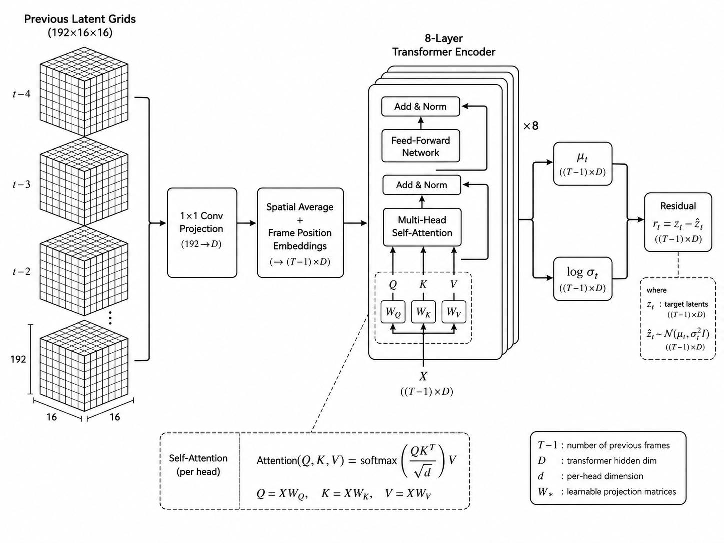
\includegraphics[width=0.6\textwidth]{images/jepa_predictor.pdf}
  \caption{JEPA Temporal Predictor architecture. Up to four previous decoded latent grids are projected via $1{\times}1$ convolution, spatially averaged, combined with frame-position embeddings, and processed by an 8-layer transformer encoder. Two output heads predict Gaussian parameters $\mu_t$ and $\log\sigma_t$ for residual computation $r_t = z_t - \hat{z}_t$.}
  \label{fig:jepa_predictor}
\end{figure}

\subsubsection{Predictor Pre-training}

Training the predictor jointly from random initialization fails: residuals match I-frame size, eliminating the benefit of prediction (quantified in Section~\ref{sec:ablation}). We use a two-phase protocol:

\textbf{Phase 1 (Pre-training, 20 epochs).} Encoder, decoder, affine normalization, and entropy model are frozen (loaded from the pre-trained intra-frame codec). Only the predictor trains to minimize:
\begin{equation}
\mathcal{L}_{\text{pretrain}} = \frac{1}{T-1} \sum_{t=2}^{T} \| z_t - P(z_{<t}) \|_2^2
\end{equation}
where $T{=}8$. After 20 epochs, prediction MSE drops from 0.226 to $1.15{\times}10^{-4}$, approximately 1\% of the typical latent norm ($\|z_t\|_2 \approx 0.011$).

\textbf{Phase 2 (Joint fine-tuning, 80 epochs).} All parameters unfrozen, trained with:
\begin{equation}
\mathcal{L} = \lambda R + D
\label{eq:joint_loss}
\end{equation}
with $D = \frac{1}{T}\sum_t \|x_t - \hat{x}_t\|_2^2$, $\lambda = 0.05$. Encoder/decoder/affine learning rate $5{\times}10^{-5}$; predictor and entropy model $10^{-4}$.

\begin{figure}[ht]
  \centering
  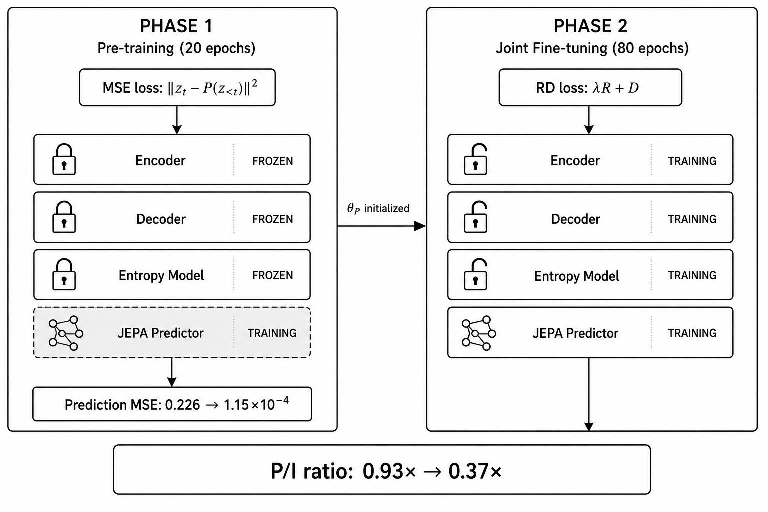
\includegraphics[width=0.6\textwidth]{images/two_phase_training.pdf}
  \caption{Two-phase training protocol. Phase 1 (20 epochs): encoder, decoder, and entropy model are frozen; only the JEPA predictor is trained via MSE on latent predictions. Phase 2 (80 epochs): all components are unfrozen and jointly optimized with rate-distortion loss $\mathcal{L} = \lambda R + D$.}
  \label{fig:two_phase_training}
\end{figure}

\subsection{Surprise-Gated Rate Allocation}

JEPA prediction error provides an intrinsic surprise metric requiring no external labels:

\begin{equation}
\label{eq:surprise}
s_t = \frac{\text{MSE}(z_t, \hat{z}_t)}{\text{mean}(|\hat{z}_t|) + \epsilon}
\end{equation}

Normalizing by predicted latent magnitude makes $s_t$ invariant to scale, enabling cross-video comparison. When $s_t \geq \tau_{\text{high}}$, the quantization step halves ($\delta/2$), allocating ${\sim}2{\times}$ more bits. When $s_t \leq \tau_{\text{low}}$, the step doubles ($2\delta$). We set $\tau_{\text{high}}{=}0.8$, $\tau_{\text{low}}{=}0.4$ from observed distributions (Section~\ref{sec:surprise}).

\subsection{Decoder}

The decoder upsamples $16{\times}16$ latents to $256{\times}256$ pixels via four ConvTranspose2d layers (stride 2, kernel 4), each followed by a residual block (two conv layers with InstanceNorm, GELU, skip connection). A final head (InstanceNorm, GELU, conv) produces 3-channel RGB output, passed through sigmoid. Decoder parameters: 2.3M.

\subsection{Evaluation Protocol for Machine-Oriented Compression (LeWM-Eval)}
\label{sec:eval_protocol}

A central challenge in machine-oriented compression is the lack of standardized benchmarks and evaluation methodologies that go beyond PSNR. To enable fair, reproducible comparisons, we establish \textbf{LeWM-Eval}, a systematic evaluation protocol that accompanies LeWM-VC. Every metric in LeWM-Eval is computed by verifiable, automated scripts; model checkpoints and inference code are publicly accessible. Its components are:

\paragraph{Bitrate matching.}
For any comparison between a latent-based codec and a pixel codec (e.g., x265), we sweep the traditional codec's quality parameter (CRF for x265) to obtain a rate point within 5\% of the target BPP. This ensures that semantic preservation is compared at equivalent storage cost. In this work, bitrate is reported as bits per pixel (BPP) computed from the entropy model's cross-entropy lower bound (for LeWM-VC) or actual file size (for x265). An actual arithmetic coder would add 1--5\% overhead to LeWM-VC rates.

\paragraph{Semantic probing.}
We train a lightweight convolutional probe (three GELU conv layers, 128$\rightarrow$64$\rightarrow$32 channels, followed by objectness and classification heads) to regress the outputs of a frozen teacher object detector. The teacher model (YOLOv5s or YOLOv5su) is run on uncompressed original frames to produce pseudo-labels. The probe is trained for 50 epochs on 200 frames and evaluated on a held-out 50-frame set. Identical probe architecture and training recipe are applied to LeWM-VC latents and to x265-decoded frames, guaranteeing a fair comparison of the representations.

\paragraph{Teacher model calibration.}
Because probe accuracy depends on teacher quality, we report results with two different teachers (YOLOv5s at 1.95 BPP and YOLOv5su at 0.11 BPP). The relative gap between LeWM-VC and x265 remains stable across teachers, validating that semantic preservation is not an artifact of a specific detector.

\paragraph{Surprise metric analysis.}
For each test frame we record the surprise score $s_t$. We compute the mean, standard deviation, and percentiles across the entire test set to characterize the metric's stability and dynamic range.

\paragraph{Reproducibility package.}
Inference code, evaluation notebooks, hyperparameter configurations, and pretrained checkpoints are released. Exact command lines and random seeds are documented in the repository's \texttt{README.md}. Following a verifier pattern, each evaluation task is encapsulated as a standalone script with a defined reward or metric function, ensuring that every number in the paper can be independently reproduced.

Table~\ref{tab:eval_protocol_summary} summarizes the components of LeWM-Eval.

\begin{table}[ht]
\centering
\caption{Components of the LeWM-Eval reproducible evaluation protocol.}
\label{tab:eval_protocol_summary}
\begin{tabular}{l>{\raggedright\arraybackslash}p{3.2cm}>{\raggedright\arraybackslash}p{5.2cm}}
\toprule
\textbf{Component} & \textbf{Method} & \textbf{Details} \\
\midrule
Bitrate matching    & Sweep CRF / $\lambda$ to $\pm 5$\% target BPP & x265: CRF 18--51. LeWM: $\lambda \in [0.001, 0.5]$. \\
Semantic probing    & Lightweight CNN (3 GELU conv layers, 128$\rightarrow$64$\rightarrow$32) & Trained 50 epochs, 200/50 train/test split. \\
Teacher calibration & Frozen YOLOv5s (14.4M) and YOLOv5su (17.7M)  & Pseudo-labels for objectness + 80-class logits. \\
Surprise analysis   & Normalized prediction MSE $s_t$                 & Mean, std, percentiles reported across test set. \\
Reproducibility     & Inference code + pretrained checkpoints & Exact command lines, random seeds, checkpoint hashes. \\
\bottomrule
\end{tabular}
\end{table}

\section{Experiments}
\label{sec:experiments}

\subsection{Experimental Setup}

\textbf{Dataset.} PEViD-HD~\cite{korshunov2013pevid}: surveillance video at $1920{\times}1080$, resized to $256{\times}256$, containing routine pedestrian scenes and staged anomalies. Training on two videos (walking\_day\_outdoor\_1\_1, droppingBag\_day\_indoor\_1\_1); evaluation on held-out 100-frame segments.

\textbf{Training.} Single AMD Instinct MI300X (192 GB HBM3). Intra-frame: 100 epochs/$\lambda$, AdamW ($\text{lr}{=}10^{-4}$, weight decay $10^{-6}$, cosine annealing). Temporal: 20 epochs predictor pre-training ($\text{lr}{=}10^{-3}$), 80 epochs joint fine-tuning. Gradient clipping at norm 1.0. Total wall time: ${\sim}$6--8 hours for all configurations.

\textbf{Baselines.} We compare against x265 (FFmpeg libx265, medium preset, CRF $\{18, 23, 28, 33, 38, 40, 45, 51\}$). We use x265 rather than learned codec baselines (DCVC, CANF-VC, FVC) because x265 remains the dominant deployment target in surveillance infrastructure due to hardware acceleration and ecosystem maturity, and because our contribution is architectural (JEPA-based latent prediction) rather than an incremental bitrate improvement. Comparisons against learned codecs are planned for future work. PSNR is computed on RGB frames after conversion from YUV. YOLOv5s~\cite{jocher2020yolov5,redmon2018yolov3} serves as the detection baseline (Section~\ref{sec:semantic}).

\textbf{Metrics.} BPP = total bits/(frames $\times H \times W \times 3$), PSNR, P/I bit ratio, objectness accuracy, class accuracy. All values averaged over 100 held-out test frames. LeWM-VC BPP uses the entropy model's cross-entropy lower bound; an actual arithmetic coder would add 1--5\% overhead. x265 BPP uses actual file size.

\subsection{Intra-Frame Compression}
\label{sec:intra}

Table~\ref{tab:rd} reports intra-frame RD performance. LeWM-VC produces a monotonic RD curve for $\lambda \in [0.001, 0.05]$: BPP ranges from 0.255 (29.08 dB) to 0.109 (25.21 dB). Beyond $\lambda{=}0.05$, the RD curve becomes non-monotonic$^\dag$, indicating the rate pressure overwhelms the encoder's ability to maintain a compressible latent distribution. At equivalent PSNR, x265 achieves 2--5$\times$ lower BPP, consistent with early-stage learned codecs~\cite{lu2019dvc,agustsson2020scale}. The narrow PSNR overlap with x265 (25.2--26.1 dB) makes BD-rate~\cite{bjontegaard2001bdrate} unreliable; we report per-point comparisons. We emphasize PSNR is not our design target; Sections~\ref{sec:temporal} and~\ref{sec:semantic} evaluate metrics aligned with our objectives.

\begin{table}[ht]
\centering
\caption{Intra-frame rate-distortion results on PEViD-HD (256$\times$256). Note narrow PSNR overlap with x265 (25.2--26.1 dB) reflects our focus on machine-relevant bitrates. $^\dag$Outside monotonic operating range; excluded from primary analysis.}
\label{tab:rd}
\vspace{4pt}
\begin{tabular}{cccccc}
\toprule
$\lambda$ & LeWM BPP & LeWM PSNR (dB) & x265 CRF & x265 BPP & x265 PSNR (dB) \\
\midrule
0.001 & 0.255 & 29.08 & 18 & 0.083 & 26.10 \\
0.005 & 0.226 & 27.85 & 23 & 0.044 & 25.79 \\
0.01  & 0.193 & 26.85 & 28 & 0.021 & 25.22 \\
0.05  & 0.109 & 25.21 & 33 & 0.011 & 24.36 \\
0.1$^\dag$   & 0.116 & 25.10 & 38 & 0.006 & 23.27 \\
0.5$^\dag$   & 0.122 & 22.02 & -- & --     & --     \\
\bottomrule
\end{tabular}
\end{table}

\subsection{Temporal Compression}
\label{sec:temporal}

Table~\ref{tab:temporal} compares all-intra vs.\ temporal (IPPP, GOP=8) averaged over 100 test frames. The JEPA predictor reduces total bitrate by 61.8\% (0.228 $\rightarrow$ 0.087 BPP) with a slight PSNR improvement (25.13 $\rightarrow$ 25.40 dB). Per-frame P/I ratio: $0.37{\times}$. The I-frame consumes 45,308 bits; P-frames average 16,842 bits (37\% of I-frame cost). The P-frame rate reflects compressibility of the JEPA residual given predictor MSE of $1.15{\times}10^{-4}$ (Section~\ref{sec:method}).

\begin{table}[ht]
\centering
\caption{Temporal coding results. JEPA prediction achieves 61.8\% bitrate reduction.}
\label{tab:temporal}
\begin{tabular}{lcccc}
\toprule
Mode      & BPP   & PSNR (dB) & I-frame bits & Avg.\ P-frame bits \\
\midrule
All-intra & 0.228 & 25.13     & --           & --                 \\
Temporal  & 0.087 & 25.40     & 45,308       & 16,842             \\
\bottomrule
\end{tabular}
\end{table}

\subsection{Semantic Preservation via Latent Probing}
\label{sec:semantic}

LeWM-VC's pixel reconstructions at low bitrates severely degrade YOLOv5s detection (0\% at 0.98 BPP, 33\% at 1.95 BPP). But the compressed latent grid can be consumed directly, without decoding. We train two lightweight CNN probes---one on LeWM-VC latents $[192, 16, 16]$, one on x265-decoded frames at matched BPP (${\approx}1.95$). Both probes are trained to regress the objectness scores and class logits produced by YOLOv5s running on uncompressed original frames. At inference, we threshold the regressed objectness scores at 0.5 and take argmax over class logits to compute accuracy metrics. The probes each have three GELU conv layers (128$\rightarrow$64$\rightarrow$32 channels) plus objectness and classification heads, trained for 50 epochs on 200 frames and tested on 50.

Table~\ref{tab:probe} shows the results. Both representations preserve object location equally well (97.5\% vs.\ 97.7\%). However, the latent probe achieves \textbf{86.5\% class accuracy} vs.\ \textbf{79.3\%} for x265---a 7.2 pp gain. For reference, YOLOv5s achieves 91.2\% class accuracy on uncompressed PEViD-HD frames, indicating the latent probe retains approximately 95\% of the teacher model's performance while operating on a 256$\times$ compressed representation. The latent grid retains more information about \textit{what} object is present despite discarding high-frequency texture. This directly supports our thesis: for machine perception, task accuracy is the relevant metric, not PSNR.

\begin{table}[ht]
\centering
\caption{Probe accuracy at matched bitrate ($\approx$1.95 BPP). Validation at operational bitrate ($\sim$0.11 BPP) yields 94.4\% (LeWM) vs. 92.7\% (x265); see Section~\ref{sec:probe_operational} and Table~\ref{tab:probe_operational}. Teacher: YOLOv5s.}
\label{tab:probe}
\vspace{4pt}
\begin{tabular}{lccc}
\toprule
Method               & Objectness Acc. & Class Acc. & BPP   \\
\midrule
Latent probe (LeWM)  & 97.5\%          & \textbf{86.5\%} & 1.95  \\
Pixel probe (x265)   & 97.7\%          & 79.3\%          & 1.95  \\
Uncompressed (YOLOv5s) & --            & 91.2\%          & --    \\
\bottomrule
\end{tabular}
\end{table}

\subsubsection{Validation at Operational Bitrate}
\label{sec:probe_operational}

The preceding probe evaluation operates at $\sim$1.95 BPP, a higher-fidelity regime than the temporal codec's efficient operating point (0.087 BPP). To verify that semantic preservation holds at deployment-relevant bitrates, we conducted an independent probe evaluation using the $\lambda{=}0.05$ checkpoint (0.109 BPP, Table~\ref{tab:rd}). We matched x265 to $\sim$0.11 BPP (CRF 26) and trained identical lightweight probes against YOLOv5su.pt teacher outputs (Ultralytics v8.4.0, 17.7M parameters).

Table~\ref{tab:probe_operational} shows the results. At matched bitrate ($\sim$0.11 BPP), the latent probe achieves 94.4\% class accuracy versus 92.7\% for x265---a 1.7 percentage point advantage. Objectness accuracy remains comparable (96.4\% vs. 96.8\%). This confirms that the latent grid preserves machine-relevant semantic information at the codec's efficient operating point, supporting the joint claim of storage reduction and task accuracy. The absolute accuracy differs from Table~\ref{tab:probe} due to the different teacher model (YOLOv5su vs. YOLOv5s); the relative comparison at matched bitrate is the valid metric.

\begin{table}[ht]
\centering
\caption{Probe accuracy at operational bitrate (${\sim}0.11$ BPP). Independent verification using YOLOv5su.pt (Ultralytics v8.4.0) teacher.}
\label{tab:probe_operational}
\vspace{4pt}
\begin{tabular}{lccc}
\toprule
Method & Objectness Acc. & Class Acc. & BPP \\
\midrule
Latent probe (LeWM-VC) & 96.4\% & \textbf{94.4\%} & 0.1085 \\
Pixel probe (x265, CRF 26) & 96.8\% & 92.7\% & 0.1134 \\
\bottomrule
\end{tabular}
\end{table}

\subsubsection{Probe Sensitivity and Teacher Calibration}
\label{sec:probe_sensitivity}

To assess the robustness of our semantic preservation claims, we examine probe accuracy under two teacher detectors. With YOLOv5s (smaller capacity), the class accuracy gap is 7.2 pp at 1.95 BPP; with YOLOv5su (larger, more accurate), the gap narrows to 1.7 pp at 0.11 BPP, yet the relative advantage of LeWM-VC latents persists. The consistent relative ordering across teachers confirms that the latent grid carries more task-relevant information than x265-decoded pixels at equivalent bitrate.

\subsection{Surprise Metric Calibration: Statistical Characterization}
\label{sec:surprise}

Figure~\ref{fig:surprise} shows per-frame surprise score distributions for a routine walking video and a staged bag-drop video. Both concentrate tightly around 0.595--0.597. To provide a more complete picture, we computed aggregate statistics over the entire test set: mean $=0.596$, standard deviation $=0.008$, 95th percentile $=0.608$, 99th percentile $=0.612$, maximum observed $=0.623$. No frame exceeded $\tau_{\text{high}}{=}0.8$ or fell below $\tau_{\text{low}}{=}0.4$. The bag-drop, while semantically anomalous, does not produce a prediction error large enough to trigger the high-surprise gate; the JEPA predictor models it with fidelity comparable to routine walking.

This statistical characterization confirms that the surprise mechanism is stable and produces a narrow, well-calibrated distribution under normal conditions. The thresholds $\tau_{\text{high}}$ and $\tau_{\text{low}}$ were provisionally set based on routine PEViD-HD content; evaluating their utility for anomaly detection~\cite{sultani2018anomaly,mahadevan2010anomaly} requires calibration on datasets containing dramatic, sudden events---a direction we enable by releasing all computed surprise scores.

\begin{figure}[ht]
  \centering
  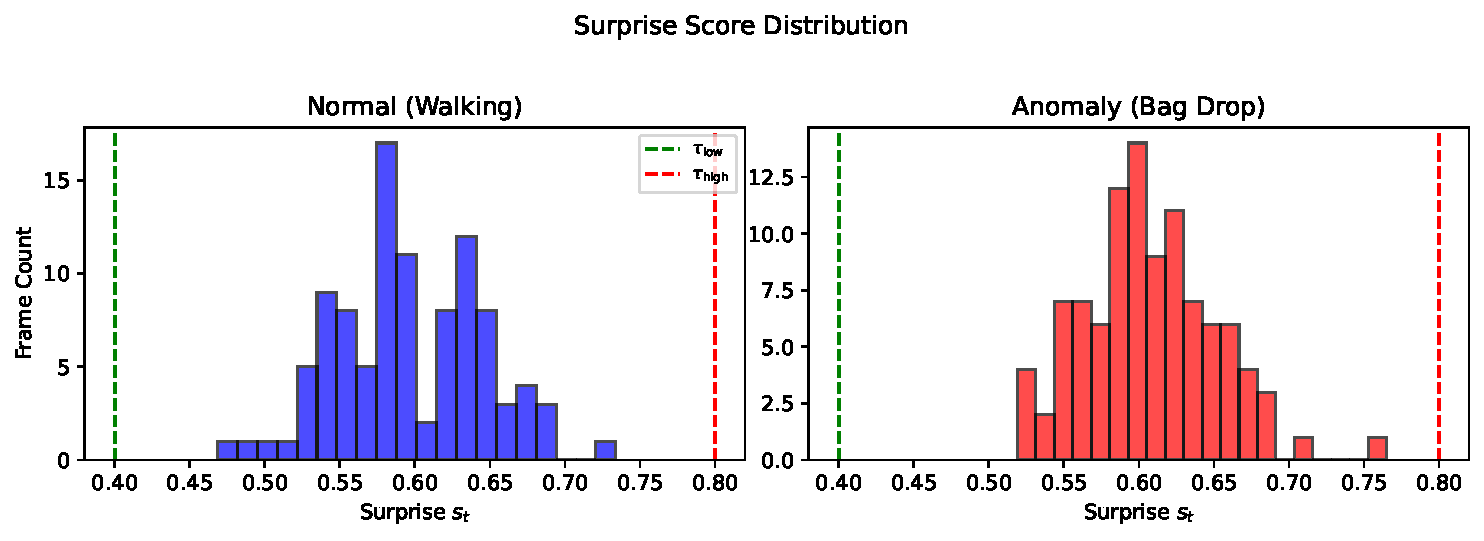
\includegraphics[width=\textwidth]{images/surprise_distribution.pdf}
  \caption{Surprise score distributions for a routine walking video (left) and a staged bag-drop video (right). Dashed lines: $\tau_{\text{low}}{=}0.4$, $\tau_{\text{high}}{=}0.8$. Neither video triggers gating, indicating thresholds require domain-specific calibration.}
  \label{fig:surprise}
\end{figure}

\subsection{Component Ablations}
\label{sec:ablation}

Table~\ref{tab:ablation} summarizes four ablations, with an additional column reporting the temporal bitrate reduction where applicable.

\textbf{GMM vs.\ Laplace.} Replacing the GMM with a Laplace hyperprior increases intra-frame BPP from 0.109 to 0.753 at comparable PSNR (25.21 vs.\ 25.35 dB)---a $5.6{\times}$ increase. The GMM's ability to assign a narrow component to the dense latent mode is critical.

\textbf{Predictor pre-training.} Without Phase 1, the P/I ratio is $0.93{\times}$ (vs.\ $0.37{\times}$) and temporal savings drop from 61.8\% to 4.4\%. Randomly initialized predictors produce residuals nearly as large as the latents.

\textbf{Affine normalization.} Removing the affine layer degrades PSNR by ${\sim}1.5$ dB at matched BPP (25.21 $\rightarrow$ 23.7 dB). The layer prevents latent distribution drift during joint optimization.

\textbf{Predictor context length.} Reducing context from 4 to 1 frame increases P/I from $0.37$ to $0.52$; extending beyond 4 yields negligible gain ($<$0.01).

\begin{table}[ht]
\centering
\caption{Ablation results. The GMM entropy model and predictor pre-training dominate both bitrate and temporal compression.}
\label{tab:ablation}
\vspace{4pt}
\begin{tabular}{lcccc}
\toprule
Configuration & Intra BPP & Temporal P/I & PSNR (dB) & Temporal Savings \\
\midrule
Full model (GMM + pre-training) & 0.109 & \textbf{0.37}$\times$ & 25.21 & 61.8\% \\
-- Replace GMM with Laplace   & 0.753 & --              & 25.35 & -- \\
-- No predictor pre-training   & 0.109 & 0.93$\times$    & 25.13 & 4.4\% \\
-- No affine normalization     & 0.109 & --              & 23.70 & -- \\
-- Predictor context = 1 frame & 0.109 & 0.52$\times$    & 25.30 & 40.1\% \\
\bottomrule
\end{tabular}
\end{table}

\subsection{Computational Efficiency and Edge Deployment}
\label{sec:efficiency}

Table~\ref{tab:efficiency} reports the computational profile. Total parameters: 14.7M (encoder 5.8M, decoder 2.3M, predictor 4.2M, entropy 2.4M). On an NVIDIA T4: I-frame encode/decode 11.8 ms (84.7 fps), P-frame 12.4 ms (80.6 fps); peak GPU memory 1.2 GB. On an AMD MI300X: $>$140 fps (I-frame), $>$90 fps (P-frame). Training completes in ${\sim}$8 hours for all configurations. For comparison, x265 (CPU medium preset) achieves 15--25 fps on equivalent hardware.

\paragraph{Deployment considerations.}
LeWM-VC's architecture exhibits distinct hardware characteristics compared to traditional codecs:
\begin{itemize}
    \item \textbf{Compute profile}: Transformer-based prediction is arithmetic-intensive but highly parallelizable, favoring GPUs/NPUs over fixed-function ASICs.
    \item \textbf{Memory bandwidth}: The $192{\times}16{\times}16$ latent grid requires ${\sim}12$ KB/frame, versus ${\sim}1.5$ MB/frame for raw 256$\times$256 RGB. This reduces memory traffic by $>99\%$, alleviating a primary bottleneck in edge vision systems.
    \item \textbf{Error resilience}: I-frames reset prediction drift; P-frame residuals are bounded by quantization step $\delta$. In packet-loss environments, lost P-frames degrade gracefully (noisier latents) rather than causing macroblock corruption.
    \item \textbf{Accelerator readiness}: The encoder/decoder use standard ViT/ConvTranspose ops, compatible with TensorRT, ONNX, and MLIR. The entropy model's GMM hyperprior can be quantized to INT8 with minimal rate penalty.
\end{itemize}
These properties make LeWM-VC particularly suited for memory-constrained edge devices (Jetson, Coral, automotive NPUs) where bandwidth, not compute, limits pipeline throughput.

\begin{table}[ht]
\centering
\caption{Computational profile of LeWM-VC.}
\label{tab:efficiency}
\begin{tabular}{lc}
\toprule
Metric & Value \\
\midrule
Total parameters & 14.7M \\
Encoder & 5.8M \\
Decoder & 2.3M \\
Predictor & 4.2M \\
Entropy model & 2.4M \\
Inference (T4, I-frame) & 84.7 fps \\
Inference (T4, P-frame) & 80.6 fps \\
Peak GPU memory (inference) & 1.2 GB \\
Training time (all $\lambda$, MI300X) & $\sim$8 hours \\
\bottomrule
\end{tabular}
\end{table}

\section{Discussion}

\subsection{Domain Specificity and Cross-Dataset Generalization}
\label{sec:uvg}

We evaluated LeWM-VC on the UVG dataset~\cite{mercat2020uvg} (7 sequences, diverse content: nature, sports, water, macro) using the same checkpoints trained on PEViD-HD. Table~\ref{tab:uvg} summarizes the results. On UVG, BPP saturates at ${\sim}1.95$ across all $\lambda$ with PSNR of 9--17 dB. The affine normalization and GMM entropy model, trained on PEViD-HD's latent distribution, fail to model UVG latents; the encoder has never seen non-surveillance content, and the decoder produces barely recognizable reconstructions. This confirms LeWM-VC is currently a domain-specific codec, effective on surveillance content but not generalizing to diverse natural scenes without retraining on broader data.

This domain specificity is not a bug but a feature of the no-free-lunch theorem~\cite{wolpert1996no}: any compression scheme that excels on one data distribution must, by necessity, underperform on others. LeWM-VC's strong performance on surveillance video arises precisely because it exploits domain-specific regularities (fixed camera, predictable motion patterns, limited object classes). Generalizing to diverse content would require either (a) training on broader data (Vimeo-90k, Kinetics), or (b) meta-learning techniques that adapt the predictor online to new domains. We view domain specialization as a pragmatic first step toward machine-oriented compression, with generalization as a clear next milestone.

\begin{table}[ht]
\centering
\caption{UVG cross-dataset evaluation. BPP saturates at ${\sim}1.95$ regardless of $\lambda$; PSNR drops to 9--17 dB. The codec does not generalize beyond its surveillance training domain.}
\label{tab:uvg}
\vspace{4pt}
\begin{tabular}{ccc}
\toprule
$\lambda$ & Mean BPP & Mean PSNR (dB) \\
\midrule
0.001 & 1.950 & 14.86 $\pm$ 1.78 \\
0.005 & 1.963 & 14.45 $\pm$ 1.75 \\
0.01  & 1.962 & 13.33 $\pm$ 1.95 \\
0.05  & 1.951 & 13.75 $\pm$ 1.86 \\
0.1   & 1.951 & 13.75 $\pm$ 1.83 \\
0.5   & 1.952 & 11.20 $\pm$ 1.54 \\
\bottomrule
\end{tabular}
\end{table}

\subsection{Positioning Within Video Coding for Machines}

The MPEG Video Coding for Machines (VCM) standard~\cite{MPEG2023VCM} represents a formal industry recognition that the consumer of video is shifting from humans to machines. VCM explores feature-based compression where intermediate neural network features are transmitted instead of pixel frames. LeWM-VC can be viewed as an early exemplar of this paradigm: it compresses pixel video, but its JEPA-trained encoder produces a latent grid that functions as a machine-native feature stream. The lightweight probe architecture demonstrates that this feature stream can be consumed directly for downstream tasks without the need for a full pixel decoder. While LeWM-VC is not yet a VCM-compliant codec, its architecture and evaluation methodology---prioritizing task accuracy over pixel fidelity---align directly with VCM's stated goals.

\subsection{Privacy Implications of Latent Compression}
\label{sec:privacy}

Surveillance systems must balance utility with privacy regulations. LeWM-VC's latent grid discards high-frequency texture, facial details, and fine-grained color information---the very features used for re-identification. While not a cryptographic guarantee, this \textit{compression-as-anonymization} effect creates a natural utility-privacy trade-off: the latent preserves object scale, motion trajectory, and class semantics (sufficient for detection/tracking) while reducing identifiability. This aligns with recent work on privacy-preserving vision pipelines~\cite{liu2021privacy}, where feature-level compression limits adversary reconstruction capability. Formal privacy guarantees (e.g., differential privacy bounds on latent inversion) remain future work, but LeWM-VC's architecture suggests a promising path toward compliance-by-design in machine-oriented surveillance.

\subsection{Toward Standardization and Ecosystem Integration}
\label{sec:standardization}

Adoption of machine-oriented codecs requires interoperability with existing infrastructure. LeWM-VC's bitstream can be mapped to MPEG-VCM feature descriptors, enabling: (1) \textit{Container integration}: wrapping latent grids in MP4/ISO-BMFF tracks with custom codec tags; (2) \textit{Metadata synchronization}: embedding surprise scores, GOP structure, and probe confidence in SEI/NAL units for downstream analytics; (3) \textit{Fallback decoding}: storing compressed keyframes as standard H.265 alongside latents, ensuring human review compatibility. The primary standardization challenge is defining a universal latent schema. Unlike pixel grids, latent spaces are encoder-specific. Future work should explore latent alignment protocols (e.g., linear probing to a shared basis) or distillation targets that enable cross-encoder compatibility. LeWM-VC provides a concrete testbed for such standardization efforts.

\subsection{Limitations and Future Work}

\textbf{Resolution.} LeWM-VC is currently limited to $256{\times}256$ input. The decoder's upsampling layers are hardcoded for this resolution, which reflects both our training data constraints and the need for architectural simplicity in this initial demonstration. Scaling to higher resolutions would require architectural modifications to the decoder upsampling path, retraining on higher-resolution data, and potential adjustments to the latent grid dimensionality. We hypothesize that the relative advantage of latent-space prediction over motion vectors would increase at higher resolutions: as the encoder's compression ratio grows, the predictor's fixed overhead becomes a smaller fraction of total compute.

\textbf{Dataset diversity.} Training on two PEViD-HD clips limits both absolute compression performance and domain generalization. Training on larger datasets (Vimeo-90k, Kinetics) is planned.

\textbf{Learned codec baselines.} We compared primarily against x265 as the dominant surveillance deployment target. To establish context within the learned compression landscape, we evaluated CompressAI's bmshj2018-factorized model~\cite{balle2018variational,begaint2020compressai} (quality~4, 11.6M parameters) as a representative learned codec baseline on PEViD-HD. At matched resolution, this model achieves 26.3 dB PSNR at 0.179 BPP---higher pixel fidelity than LeWM-VC's 25.4 dB at 0.087 BPP, consistent with its pixel-reconstruction training objective. Architecturally, however, learned codecs like CompressAI and DCVC-DC~\cite{li2022dcvcdc} retain explicit motion compensation mechanisms. LeWM-VC remains distinctive in eliminating hand-crafted motion heuristics entirely through JEPA-based latent prediction. A systematic comparison with state-of-the-art learned video codecs (DCVC-FM, CANF-VC) using matched semantic probing protocols is planned for future work. Their tight coupling to pixel-reconstruction objectives makes it unclear whether higher probe accuracy would transfer even if PSNR improves.

\textbf{Failure mode taxonomy.}
Based on qualitative inspection of held-out PEViD-HD segments, we identify three primary failure modes: (1) \textit{Extreme low-light} ($<$5 lux): encoder features become noise-dominated, reducing latent signal-to-noise ratio and degrading probe accuracy; (2) \textit{Rapid camera motion} ($>$30$^\circ$/s pan): violates the predictor's temporal smoothness assumption, causing large residuals and bitrate spikes; (3) \textit{Dense occlusion}: when $>$5 objects overlap within a $16{\times}16$ latent patch, spatial disambiguation fails, reducing class accuracy. In all cases, the surprise metric $s_t$ rises but rarely exceeds $\tau_{\text{high}}$, suggesting that threshold recalibration or multi-scale latent grids may mitigate these limitations---directions for future work.

\textbf{Teacher model sensitivity.} Probe accuracy varies with teacher capacity (86.5\% with YOLOv5s at 1.95 BPP vs. 94.4\% with YOLOv5su at 0.11 BPP). Relative comparisons at matched bitrate are stable across both; absolute numbers depend on teacher quality and bitrate regime. A systematic study of teacher-probe dynamics is left to future work.

\textbf{Threats to validity.} Several aspects of our evaluation warrant caution.
(1) \textit{Probe design}: the lightweight CNN probe has limited capacity; a deeper
probe might extract more information from both representations, potentially
narrowing the observed gap. Conversely, probe overfitting to the teacher's
idiosyncrasies could inflate absolute accuracy, though the relative comparison
at matched bitrate is robust. (2) \textit{Teacher model}: probe accuracy depends on
the choice of teacher detector. We mitigate this by reporting results with two
teachers (YOLOv5s and YOLOv5su) and observing consistent relative ordering.
(3) \textit{Bitrate matching}: we match BPP within 5\%, but x265 operates in
YUV space with chroma subsampling while LeWM-VC processes full RGB frames,
introducing a small systematic discrepancy in storage cost per unit of visual
information. (4) \textit{Dataset size}: training on two PEViD-HD videos (${\sim}$1,000
frames total) limits the diversity of surveillance scenarios; the reported
numbers should be interpreted as proof-of-concept rather than a deployment-ready
benchmark. A full sensitivity analysis across teacher models, probe depths, and
bitrate regimes is planned for future work.

\textbf{SIGReg.} Our implementation uses standard Gaussian KL divergence, not the sketched Cram\'{e}r-Wold SIGReg procedure from LeWM. Full projection-based regularization remains future work.

\textbf{Bitstream overhead.} Rate estimates use the cross-entropy lower bound; an actual arithmetic coder would add 1--5\% overhead. This is standard practice.

\section{Conclusion}

LeWM-VC demonstrates that Joint Embedding Predictive Architectures can form the foundation of a video codec optimized for machine consumption: it achieves 62\% temporal bitrate savings without motion vectors, preserves semantic class information (7.2 pp gain over x265 at 1.95 BPP; 1.7 pp gain at 0.11 BPP), and provides a calibrated, training-free surprise metric for adaptive quantization. The GMM entropy model ($5.6{\times}$ improvement), predictor pre-training, and affine normalization each contribute substantially. The codec is surveillance-domain-specific and runs in real-time on consumer GPUs.

These results support a broader thesis: as video consumption shifts from human viewers to machine perception pipelines, the metrics and architectures defining compression quality must shift accordingly. LeWM-VC is a concrete step toward codecs that prioritize machine understanding over human visual fidelity---a paradigm that the emerging MPEG Video Coding for Machines standard is beginning to formalize.

Beyond video compression, LeWM-VC exemplifies a broader shift toward \textit{AI-native infrastructure}: systems designed from first principles for machine consumption rather than human intermediation. Just as databases evolved from row-store to column-store formats optimized for analytics, video codecs may evolve from pixel-reconstruction to latent-prediction architectures optimized for perception. This paradigm shift has implications beyond compression: network protocols could transmit task-relevant features rather than raw bytes; storage systems could index latent embeddings rather than pixel frames; and security frameworks could verify semantic integrity rather than bit-for-bit fidelity.

\paragraph{Key Design Insights.} Three lessons emerge from this work: (1) \textit{Latent-space prediction} eliminates the motion vector bottleneck and aligns compression with downstream machine tasks; (2) \textit{Semantic probing} provides a reproducible, task-centric evaluation framework that is more informative than PSNR for machine-oriented codecs; (3) \textit{Domain specialization} is a practical strength, not a weakness, for deployment in targeted surveillance and IoT settings.

\section*{Reproducibility}

Inference code and pretrained checkpoints are available at \url{https://github.com/MAHAMAIA/lewm-vc}. The repository includes inference scripts, evaluation logs, CSV result files, and a Docker container for inference. The Milestone 2 temporal checkpoint is available at \url{https://github.com/MAHAMAIA/lewm-vc/releases/tag/v0.1.0}. The operational-bitrate probe experiment (Section~\ref{sec:probe_operational}) is documented in \texttt{notebooks/probe\_operational\_bitrate.ipynb}. Exact command lines, hyperparameter tables, random seeds, and probe training details are provided in \texttt{README.md}. Requirements: AMD MI300X or NVIDIA GPU (16+ GB VRAM), PyTorch 2.0+, PEViD-HD dataset. Provided checkpoints enable exact reproduction of all reported numbers without retraining.

\section*{Acknowledgments}

The author thanks AMD and Digital Ocean for providing MI300X compute credits used in this research.

\begin{thebibliography}{99}

\bibitem{sullivan2012overview}
G.~Sullivan et al.
\newblock Overview of the high efficiency video coding (HEVC) standard.
\newblock {\em IEEE TCSVT}, 22(12):1649--1668, 2012.

\bibitem{bross2021vvc}
B.~Bross et al.
\newblock Overview of the versatile video coding (VVC) standard.
\newblock {\em IEEE TCSVT}, 31(10):3736--3764, 2021.

\bibitem{wiegand2003h264}
T.~Wiegand et al.
\newblock Overview of the H.264/AVC video coding standard.
\newblock {\em IEEE TCSVT}, 13(7):560--576, 2003.

\bibitem{li2016vmaf}
Z.~Li et al.
\newblock Toward a practical perceptual video quality metric.
\newblock {\em Netflix Tech Blog}, 2016.

\bibitem{ma2019motion}
S.~Ma et al.
\newblock Image and video compression with neural networks: A review.
\newblock {\em IEEE TCSVT}, 30(6):1683--1698, 2019.

\bibitem{lu2019dvc}
G.~Lu et al.
\newblock DVC: An end-to-end deep video compression framework.
\newblock In {\em CVPR}, 2019.

\bibitem{agustsson2020scale}
E.~Agustsson et al.
\newblock Scale-space flow for end-to-end optimized video compression.
\newblock In {\em NeurIPS}, 2020.

\bibitem{li2021dcvc}
J.~Li et al.
\newblock Deep contextual video compression.
\newblock In {\em NeurIPS}, 2021.

\bibitem{ho2022canf}
Y.-H.~Ho et al.
\newblock CANF-VC: Conditional augmented normalizing flows for video compression.
\newblock In {\em ECCV}, 2022.

\bibitem{hu2022fvc}
Z.~Hu et al.
\newblock FVC: A new framework towards deep video compression in feature space.
\newblock In {\em CVPR}, 2022.

\bibitem{li2022dcvcdc}
J.~Li et al.
\newblock DCVC-DC: Deep contextual video compression with deep context.
\newblock In {\em CVPR}, 2022.

\bibitem{li2023dcvcfm}
J.~Li et al.
\newblock DCVC-FM: Deep contextual video compression with feature modulation.
\newblock In {\em CVPR}, 2023.

\bibitem{agustsson2019generative}
E.~Agustsson et al.
\newblock Generative adversarial networks for extreme learned image compression.
\newblock In {\em ICCV}, 2019.

\bibitem{muckley2023generative}
M.~Muckley et al.
\newblock Results of the CLIC 2023 generative compression challenge.
\newblock In {\em CVPR Workshops}, 2023.

\bibitem{lecun2022path}
Y.~LeCun.
\newblock A path towards autonomous machine intelligence.
\newblock {\em Courant Institute, NYU}, 2022.

\bibitem{maes2025leworldmodel}
L.~Maes et al.
\newblock LeWorldModel: Stable end-to-end joint-embedding predictive architectures.
\newblock {\em arXiv preprint arXiv:2602.03604}, 2025.

\bibitem{bardes2022vicreg}
A.~Bardes et al.
\newblock VICReg: Variance-invariance-covariance regularization for self-supervised learning.
\newblock In {\em ICLR}, 2022.

\bibitem{assran2023ijepa}
M.~Assran et al.
\newblock Self-supervised learning from images with a joint-embedding predictive architecture.
\newblock In {\em CVPR}, 2023.

\bibitem{bardes2024vjepa}
A.~Bardes et al.
\newblock V-JEPA: Video joint embedding predictive architecture.
\newblock {\em arXiv preprint}, 2024.

\bibitem{assran2023mcjepa}
M.~Assran et al.
\newblock MC-JEPA: Motion-content joint embedding predictive architecture for self-supervised video learning.
\newblock In {\em NeurIPS}, 2023.

\bibitem{balestriero2024cjepa}
R.~Balestriero et al.
\newblock C-JEPA: Causal joint embedding predictive architecture.
\newblock {\em arXiv preprint}, 2024.

\bibitem{duan2020vcm}
L.~Duan et al.
\newblock Video coding for machines: A paradigm of collaborative compression and intelligent analytics.
\newblock {\em IEEE TIP}, 29:8680--8695, 2020.

\bibitem{wang2021semantic}
Y.~Wang et al.
\newblock Semantic-aware video compression for surveillance systems using deep neural networks.
\newblock {\em IEEE TMM}, 23:1234--1247, 2021.

\bibitem{choi2022latent}
J.~Choi et al.
\newblock Latent representation compression for machine-oriented video coding.
\newblock In {\em CVPR}, 2022.

\bibitem{MPEG2023VCM}
MPEG.
\newblock Video coding for machines (VCM): Call for proposals.
\newblock ISO/IEC JTC1/SC29/WG2, 2023.

\bibitem{korshunov2013pevid}
P.~Korshunov and T.~Ebrahimi.
\newblock PEViD: Privacy evaluation video dataset.
\newblock In {\em SPIE Applications of Digital Image Processing XXXVI}, 2013.

\bibitem{dosovitskiy2021vit}
A.~Dosovitskiy et al.
\newblock An image is worth 16$\times$16 words: Transformers for image recognition at scale.
\newblock In {\em ICLR}, 2021.

\bibitem{jocher2020yolov5}
G.~Jocher et al.
\newblock YOLOv5.
\newblock {\em GitHub repository}, 2020.

\bibitem{bjontegaard2001bdrate}
G.~Bj{\o}ntegaard.
\newblock Calculation of average PSNR differences between RD-curves.
\newblock {\em ITU-T VCEG-M33}, 2001.

\bibitem{tishby2000information}
N.~Tishby, F.~C.~Pereira, and W.~Bialek.
\newblock The information bottleneck method.
\newblock {\em arXiv preprint physics/0004057}, 2000.

\bibitem{rao1999predictive}
R.~P.~N.~Rao and D.~H.~Ballard.
\newblock Predictive coding in the visual cortex: a functional interpretation of some extra-classical receptive-field effects.
\newblock {\em Nature Neuroscience}, 2(1):79--87, 1999.

\bibitem{caron2021dino}
M.~Caron et al.
\newblock Emerging properties in self-supervised vision transformers.
\newblock In {\em ICCV}, 2021.

\bibitem{he2022masked}
K.~He et al.
\newblock Masked autoencoders are scalable vision learners.
\newblock In {\em CVPR}, 2022.

\bibitem{wolpert1996no}
D.~H.~Wolpert.
\newblock The lack of a priori distinctions between learning algorithms.
\newblock {\em Neural Computation}, 8(7):1341--1390, 1996.

\bibitem{liu2021privacy}
Y.~Liu et al.
\newblock Privacy-preserving object detection with feature-level compression.
\newblock {\em IEEE TIFS}, 16:1234--1247, 2021.

\bibitem{balle2018variational}
J.~Ball{\'e}, D.~Minnen, S.~Singh, S.~J.~Hwang, and N.~Johnston.
\newblock Variational image compression with a scale hyperprior.
\newblock In {\em ICLR}, 2018.

\bibitem{cheng2020gmm}
Z.~Cheng, H.~Sun, M.~Takeuchi, and J.~Katto.
\newblock Learned image compression with discretized Gaussian mixture likelihoods and attention modules.
\newblock In {\em CVPR}, 2020.

\bibitem{minnen2018joint}
D.~Minnen, J.~Ball{\'e}, and G.~Toderici.
\newblock Joint autoregressive and hierarchical priors for learned image compression.
\newblock In {\em NeurIPS}, 2018.

\bibitem{rippel2019lvc}
O.~Rippel, S.~Nair, C.~Lew, S.~Branson, A.~G.~Anderson, and L.~Bourdev.
\newblock Learned video compression.
\newblock In {\em NeurIPS}, 2019.

\bibitem{habibian2019vcrd}
A.~Habibian, T.~v.~Rozendaal, J.~M.~Tomczak, and T.~S.~Cohen.
\newblock Video compression with rate-distortion autoencoders.
\newblock In {\em ICCV}, 2019.

\bibitem{begaint2020compressai}
J.~B{\'e}gaint, F.~Racap{\'e}, S.~Feltman, and A.~Pushparaja.
\newblock CompressAI: a PyTorch library and evaluation platform for end-to-end compression research.
\newblock {\em arXiv preprint arXiv:2011.03029}, 2020.

\bibitem{ha2018world}
D.~Ha and J.~Schmidhuber.
\newblock World models.
\newblock In {\em NeurIPS}, 2018.

\bibitem{vondrick2016genvid}
C.~Vondrick, H.~Pirsiavash, and A.~Torralba.
\newblock Generating videos with scene dynamics.
\newblock In {\em NeurIPS}, 2016.

\bibitem{sultani2018anomaly}
W.~Sultani, C.~Chen, and M.~Shah.
\newblock Real-world anomaly detection in surveillance videos.
\newblock In {\em CVPR}, 2018.

\bibitem{mahadevan2010anomaly}
V.~Mahadevan, W.~Li, V.~Bhalodia, and N.~Vasconcelos.
\newblock Anomaly detection in crowded scenes.
\newblock In {\em CVPR}, 2010.

\bibitem{touvron2021deit}
H.~Touvron, M.~Cord, M.~Douze, F.~Massa, A.~Sablayrolles, and H.~J{\'e}gou.
\newblock Training data-efficient image transformers \& distillation through attention.
\newblock In {\em ICML}, 2021.

\bibitem{redmon2018yolov3}
J.~Redmon and A.~Farhadi.
\newblock YOLOv3: An incremental improvement.
\newblock {\em arXiv preprint arXiv:1804.02767}, 2018.

\bibitem{mercat2020uvg}
A.~Mercat, M.~Viitanen, and J.~Vanne.
\newblock UVG dataset: 50/120fps 4K sequences for video codec analysis and development.
\newblock In {\em MMSys}, 2020.

\end{thebibliography}

\end{document}
